\chapter{Свойства случайных процессов}
\section*{Часть III} \textbf{Свойства случайных процессов}

\textit{Основано на \cite{adeshereKorrelyaciyaMezhduVremennymi2021},
\cite{panovTeoriyaSluchaynyhProcessov2018}}

\section{Стационарность}
\defn{Стационарность в узком смысле}{
  %\subsection*{Определение 9.1}
  Случайный процесс \( X_t \) называется
  стационарным (stationary, стационарным в узком смысле), если все его
  конечномерные распределения инвариантны относительно сдвигов, т.е.
  для любых наборов моментов времени $t1 , \ldots, tn$ , любых вещественных
  $x1 , \ldots, xn$ и любого $h > 0$:

  \[ \mathbb{P}(X_{1} \leq x_{1}, \ldots, X_{n} \leq x_{n}) =
  \mathbb{P}(X_{t_1 + h} \leq x_{1}, \ldots, X_{t_n + h} \leq x_{n}), \]
}
%\subsection*{Определение 9.2}
\defn{Стационарность в широком смысле} {
  Случайный процесс \( X_t \) называется
  стационарным в широком смысле (wide sense stationary,
    weakly stationary, covariance stationary,
  second-order stationary), если $m(t)$ является постоянной величиной
  (не зависящей от $t$), и кроме того, для любых $h > 0$, $s$, $t \in
  \mathbb{R}$ выполнено

\[ K(t + h, s + h) = K(t, s). \] }

Другими словами, процесс с постоянным математическим ожиданием
является стационарным в широком смысле тогда и только тогда, когда
существует функция $ \gamma : \mathbb{R} \to \mathbb{R} $ такая, что $
K(t, s) = \gamma(t-s) $ для любых $t$, $s$.

%\textcolor{blue}{\textbf{В контексте анализа временных рядов
%нам обычно достаточно выполнение стационарности в широком смысле}}
В контексте анализа временных рядов
нам обычно достаточно выполнение стационарности в широком смысле.

\ex{Виды стационарностей}{
1) Узкая стационарность: Все данные на все точки строго из одного
распределения.\\
2) Широкая стационарность: Первая половина элементов взята из
экспоненциального распределения, а вторая половина из нормального. Но
1 и 2 моменты у них совпадают и автоковариация зависит только от лага
=> ряд стационарен в широком смысле
}

Функция $ \gamma
(\cdot) $ называется автоковариационной функцией
(autocovariance function)
и обладает следующими свойствами.

% Добавить в вопросы для закрепления картинки . Наглядно рассмотрим виды
% различных процессов и определим их стационарность.

%\begin{figure}[htb]
%\centering
%\definecolor{myorange}{RGB}{255,165,0} % RGB для "оранжевый" % Не сработало
%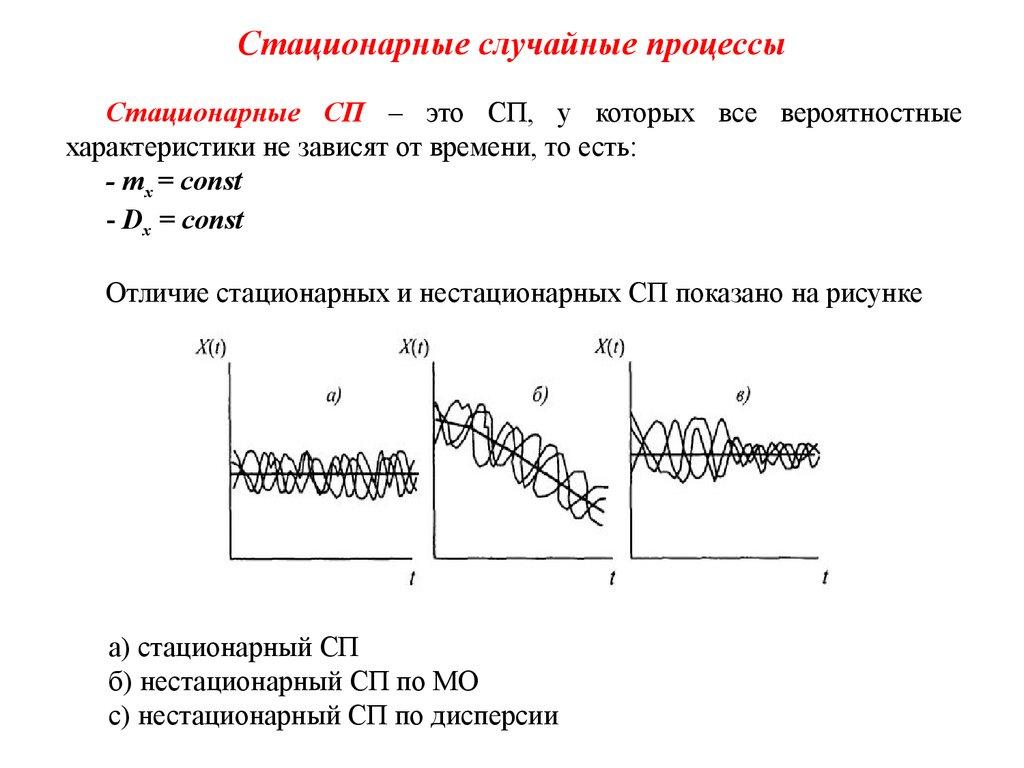
\includegraphics[width=1\textwidth]{images/stationarity.jpg}
%\textcolor{myorange}{\textbf{\caption{Figure
%Descriptiondas}}}\label{fig:1} % ЦВЕТ НЕ ОТРАБОТАЛ
%\end{figure}

%\textbf{Утверждение 9.3.} Пусть $\gamma$ — автоковариационная функция
%некоторого стационарного в широком смысле случайного процесса. Тогда
%\begin{itemize}
%\item[(i)] $\gamma(0) \geq 0$.
%\item[(ii)] $|\gamma(u)| \leq \gamma(0)$.
%\item[(iii)] $\gamma$ является четной функцией.
%\end{itemize}

\asum{Свойства автоковариационной функции}{Пусть $\gamma$ —
автоковариационная функция
некоторого стационарного в широком смысле случайного процесса. Тогда
\begin{itemize}
\item[(i)] $\gamma(0) \geq 0$.
\item[(ii)] $|\gamma(u)| \leq \gamma(0)$.
\item[(iii)] $\gamma$ является четной функцией.
\end{itemize}}

\section{Эргодичность}
Понятие эргодичности мотивировано законом больших чисел. Рассмотрим процесс
$X_t$, наблюдаемый в дискретные моменты времени $t = 1, 2, \ldots, T$
и зададимся вопросом, сходится ли процесс \[ M_T = \frac{1}{T}
\sum_{t=1}^{T} X_t \] при устремлении горизонта времени $T \to
\infty$.

\defn{} {Процесс $X_t$ с дискретными
временами $t = 1, 2, \ldots$ называется \textit{эргодическим по
среднему}, если \[ M_T
\xrightarrow{p} \mu, \quad \text{при } T \to \infty \] где $\mu$ —
некоторая константа.}

\begin{figure}[H]
\centering
\definecolor{myorange}{RGB}{255,165,0} % RGB для "оранжевый" % Не сработало
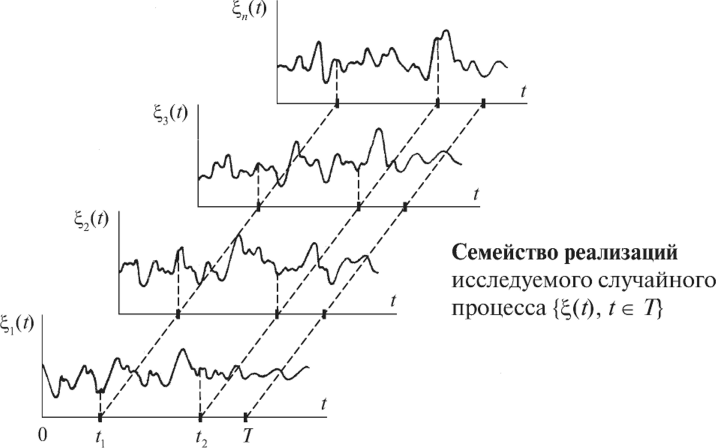
\includegraphics[width=1\textwidth]{images/ch2_ergodicity.png}
{\textbf{\caption{Семейство реализаций СП}}}\label{fig:2} % ЦВЕТ НЕ ОТРАБОТАЛ
\end{figure}

Давайте вернемся к тому, с чего начинали. Во введении мы говорили о
необходимости иметь множество реализаций случайного процесса для
того, чтобы иметь возможность адекватно посчитать по ним статистики.
Оказывается, что для эргодических случайных
процессов, все характеристики которых неизменны во времени, наличие
ансамбля не обязательно! То есть, нам не потребуется десять
реализаций, чтобы оценить какую-нибудь статистику. Вместо этого
достаточно некоторое время понаблюдать за одной! Например, чтобы
оценить коэффициент корреляции между X и Y, достаточно иметь одну
реализацию X и еще одну – Y. Что, собственно, все мы и делаем,
когда вычисляем коэффициент корреляции между потеплением и
пиратами.

%При анализе наблюдений очень часто априори считается, что исследуемые
%процессы являются эргодическими. Иногда это даже не оговаривается специально.

%\case{
При анализе наблюдений очень часто
априори считается, что исследуемые
процессы являются эргодическими. Иногда это даже не оговаривается специально.
%}
%\theorem{dsa}{
Но если мы хотим избежать грубейших ошибок, то нельзя
забывать, что
гипотеза эргодичности – это только гипотеза.
%}

%\theoremr{gs}{kzk}
%Но если мы хотим избежать грубейших ошибок, то нельзя забывать, что
%гипотеза эргодичности – это только гипотеза.

Подавляющее
большинство долговременных наблюдений продолжается конечное время
(вы поняли, это такая шутка), а на выходе получается единственный
ряд. Доказать эргодичность такого процесса в принципе невозможно.
Поэтому, начиная анализ данных, мы чаще всего просто постулируем ее
явным образом или неявно. А что еще остается делать, если в наличии
куча данных и руки чешутся начальник требует срочно использовать
всю мощь безупречного, многократно проверенного теоретиками
статистического инструментария для достижения практических целей?

На самом деле, подавляющее большинство временных рядов вовсе
не являются эргодическими. И если доказать эргодичность процесса
достаточно сложно (практически нереально), то вот
опровергнуть ее часто можно без особых усилий. Достаточно просто
вспомнить, что практически все экспериментальные временные ряды
существенно нестационарны. Огромный массив накопленных
экспериментальных данных однозначно свидетельствует, что априорная
"базовая модель" почти любого природного процесса – это вовсе не
белый шум (для которого действительно можно заигрывать с
эргодичностью). Нет, спектры большинства реальных сигналов имеют
степенной вид (Точнее, они обычно становятся степенными после
удаления доминирующих периодичностей - сезонной, суточной и т.д.)

Но если ряд не стационарен, то он заведомо не может
рассматриваться, как последовательность измерений одной и той же
случайной величины. Для него совершенно бессмысленно оценивать те
статистики, которые вводятся и исследуются при анализе случайных величин.

Из стационарности не следует эргодичность.

% TODO: вынести в bib файл
% Рис 2.1
% (https://studref.com/705179/tehnika/svoystvo_ergodichnosti_sluchaynyh_protsessov)
% Набросок 2.x.1 (https://en.ppt-online.org/73629)

%\section*{Пример}
\ex{Расммотрим некоторый случайный процесс и проверим его свойства}
{

Пусть \( X(t) \) — белый шум со случайной мощностью, заданный в виде:
\[
X(t) = \sigma \cdot W(t),
\]
где:
\begin{itemize}
\item \( W(t) \) — стандартный белый шум в дискретном времени \(t
  \in \mathbb{Z}\), \(
  E[W(t)] = 0 \), единичной дисперсией \( \text{Var}[W(t)] = 1 \),
  и автокорреляцией \( R_W(\tau) = \delta(\tau) \),

  \footnote{Функция Дирака $\delta(\tau)$ определяется как
    $\delta(0)=1$ и $\delta(\tau)=0$ при $\tau \neq 0$ в дискретном
    случае; в непрерывном времени это обобщённая функция (дистрибуция)
  с $\int \delta(\tau) d\tau = 1$.}

\item \( \sigma \) — случайная величина, не зависящая от \( W(t)
  \), с \( E[\sigma^2] < \infty \).
\end{itemize}

%\section*{Доказательство стационарности}
\textbf{1.Сначала докажем стационарность процесса:}\\
\textit{Для этого вспомним условие стационарности в широком смысле:}

%\textbf{Условия стационарности в широком смысле:}
\begin{itemize}
\item Среднее не зависит от времени:
  \[
    E[X(t)] = E[\sigma \cdot W(t)] = E[\sigma] \cdot E[W(t)] = 0.
  \]

\item Автокорреляционная функция зависит только от разности \( \tau
  = t_1 - t_2 \):
  \[
    R_X(t_1, t_2) = E[X(t_1)X(t_2)] = E[\sigma^2 W(t_1) W(t_2)] =
    E[\sigma^2] \cdot \delta(t_1 - t_2).
  \]
  Обозначим \( R_X(\tau) = E[\sigma^2] \delta(\tau) \), что зависит
  только от \( \tau \).
\end{itemize}

\textbf{Вывод:}\\
Процесс \( X(t) \) \textbf{стационарен}, так как его среднее
постоянно, а автокорреляция зависит только от временного сдвига.\\

\textbf{2. Далее докажем его неэргодичность:}\\

%\subsection*{Среднее значение}
\textit{2.1 Среднее значение:}
\begin{itemize}
  %\item \textbf{По ансамблю:} \( E[X(t)] = 0 \) (доказано выше).
  %\item \textbf{По времени (для одной реализации):}
\item {По ансамблю:} \( E[X(t)] = 0 \) (доказано выше).
\item {По времени (для одной реализации):}
  \[
    \lim_{T \to \infty} \frac{1}{T} \int_{-T/2}^{T/2} X(t) \, dt =
    \sigma \cdot \lim_{T \to \infty} \frac{1}{T} \int_{-T/2}^{T/2}
    W(t) \, dt = 0 \quad \text{(т.к. \( W(t) \) имеет нулевое среднее)}.
  \]
  Здесь совпадение есть.
\end{itemize}

%\subsection*{Дисперсия (второй момент)}
\textit{2.2 Дисперсия (второй момент):}
\begin{itemize}
  %\item \textbf{По ансамблю:}
\item {По ансамблю:}
  \[
    E[X^2(t)] = E[\sigma^2 W^2(t)] = E[\sigma^2] \cdot E[W^2(t)] =
    E[\sigma^2] \cdot \delta(0).
  \]
  (Для дискретного белого шума \( \delta(0) = 1 \), для
  непрерывного — обобщённая функция.)

  %\item \textbf{По времени (для одной реализации):}
\item {По времени (для одной реализации):}
  \[
    \lim_{T \to \infty} \frac{1}{T} \int_{-T/2}^{T/2} X^2(t) \, dt
    = \sigma^2 \cdot \lim_{T \to \infty} \frac{1}{T}
    \int_{-T/2}^{T/2} W^2(t) \, dt = \sigma^2 \cdot E[W^2(t)] = \sigma^2.
  \]
  Но \( \sigma^2 \) — случайная величина, а не константа \( E[\sigma^2] \).
\end{itemize}

\textbf{Вывод:}
\begin{itemize}
\item Для \textbf{среднего} эргодичность есть.
\item Для \textbf{дисперсии (и более высоких моментов)}
  эргодичности \textbf{нет}, так как усреднение по времени даёт \(
  \sigma^2 \), а не \( E[\sigma^2] \).
\end{itemize}
}

\question{Свойства случайных процессов}{
\item Что такое стационарность в узком и широком смысле?
\item Зачем нужна стационарность? Какие из алгоритмов машинного
обучения требуют стационарности исходных данных?
\item Как визуально на основании графика определить, является ли
процесс стационарным
}

\printbibliography[heading=subbibliography, title={Источники}]
